\section{Grundlagen}

\subsection{Einheiten}

Korrekte Angabe von Werten:\\
\noindent
\begin{minipage}{0.5\columnwidth}
    % LTeX: enabled=false
\begin{tikzpicture}
    \node (value) {12};
    \node [right=0.0cm of value] (prefix) {$\text{\textmu}$};
    \node [right=0.0cm of prefix] (unit) {$\si{\m}$};
    \draw[->] 
    (value.south) -- ++(0,-1.25)
               -- ++(1.4,0)
               node[anchor=west] {Wert};
    \draw[->]
    (prefix.south) -- ++(0,-0.75)
               -- ++(0.9,0)
               node[anchor=west] {Präfix};
    \draw[->]
    (unit.south) -- ++(0,-0.25)
               -- ++(0.5,0)
               node[anchor=west] {Einheit};
    
\end{tikzpicture}
\end{minipage}
\begin{minipage}{0.5\columnwidth}
    \{x\} $\rightarrow$ Zahlenwert = 12\\
    $[x]$ $\rightarrow$ Einheit abrufen = \unit{\kilo\gram\metre\per\square\second}$\rightarrow$ kann präfixe enthalten ist technisch gesehen nicht ganz richtig\\
\end{minipage}

\subsection{Graphen}
\begin{center}
    % LTeX: enabled=false
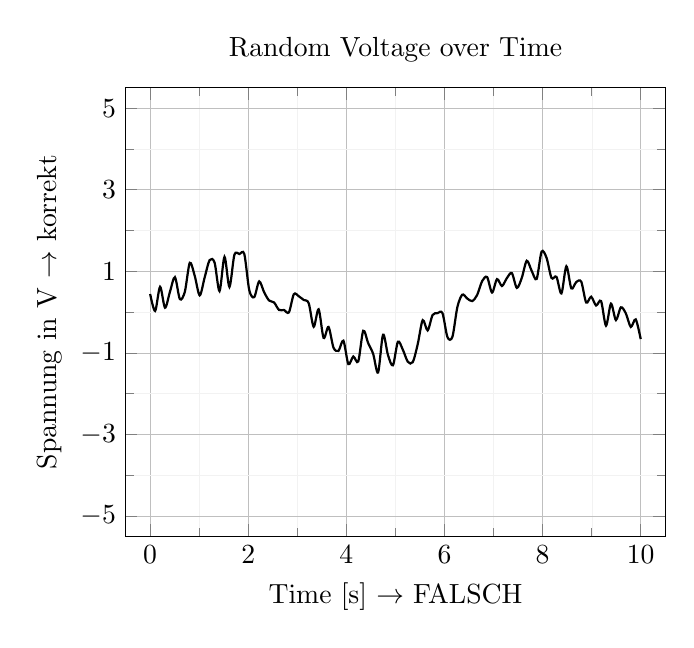
\begin{tikzpicture}
    \begin{axis}[
        title={Random Voltage over Time},
        xlabel={Time [s] $\rightarrow$ FALSCH},
        ylabel={Spannung in V $\rightarrow$ korrekt},
        xmin=0, xmax=10,
        ymin=-5, ymax=5,
        xtick={0,2,4,6,8,10},
        ytick={-5,-3,...,5},
        grid=both,
        grid style={line width=.1pt, draw=gray!10},
        major grid style={line width=.2pt,draw=gray!50},
        minor tick num=1,
        enlarge x limits={abs=0.5},
        enlarge y limits={abs=0.5},
        axis background/.style={fill=white},
        legend style={at={(0.5,-0.1)},anchor=north},
        no markers,
        every axis plot/.append style={thick}
    ]
    
    \addplot[
        domain=0:10,
        samples=100,
        smooth,
    ] {sin(deg(x)) + rand*0.5};
    
    \end{axis}
\end{tikzpicture}
\end{center}
Für Graphen muss darauf geachtet werden das die Einheit korrekt angegeben wird. 
Die Angabe in Eckigen klammern ist nicht mehr zu verwenden. 
